\documentclass[a4paper, 12pt]{article}
\usepackage{template/sleek-settings}

% DEFAULT MARDKOWN SETUP

% TIGHTLIST UPDATE
\providecommand{\tightlist}{\setlength{\itemsep}{0pt}\setlength{\parskip}{0pt}}

\RequirePackage[
unicode=true,
breaklinks=true,
pdfusetitle,
linktoc=page,
linkbordercolor=blue,
            linkbordercolor=black,
        citebordercolor=blue,
        urlbordercolor=black,
        pdfborder={.5 .5 .5}
    ]{hyperref}








\urlstyle{same}

% END OF DEFAULT MARKDOWN SETUP
% DYNAMIC VARIABLES

\title{LSTAT2130 - Bayesian Statistics}

\subtitle{Project - Group Q}

\author{ \textsc{Lionel Lamy - 1294-1700}\\  \textsc{Adrien
Kinart}\\  \textsc{Simon Lengendre}\\ }

\logo{resources/img/UCLouvainLogoSciences.jpg}

\institute{Université catholique de Louvain}

\faculty{Louvain School of Statistics}



\date{\today}

\setcounter{tocdepth}{3}

% END OF DYNAMIC VARIABLES

\begin{document}

    \maketitle
    \tableofcontents
    \newpage
    
        
    
    \hypertarget{introduction}{%
    \section{Introduction}\label{introduction}}

\begin{verbatim}
##    shape 
## 3089.944
\end{verbatim}

\begin{verbatim}
##    shape 
## 0.399687
\end{verbatim}

    \begin{center}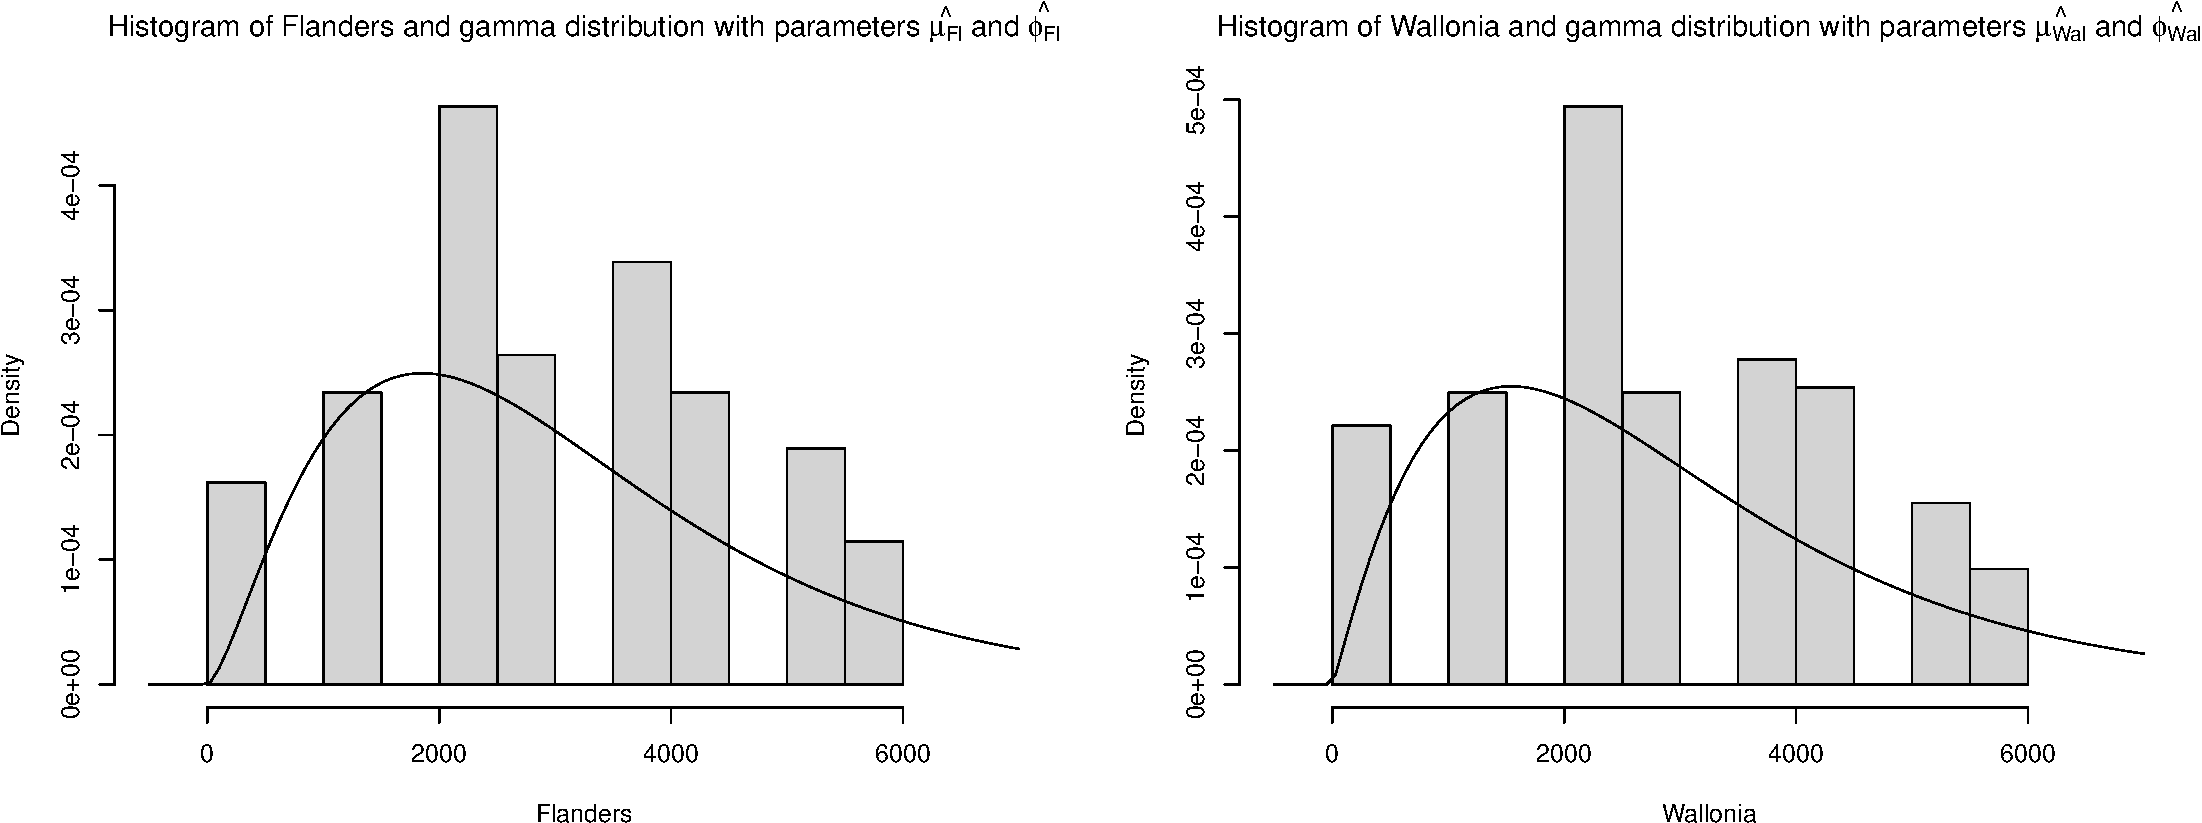
\includegraphics[width=0.8\linewidth]{resources/figs/flanders_wallonia-1} \end{center}

\begin{verbatim}
##    shape 
## 2914.882
\end{verbatim}

\begin{verbatim}
##    shape 
## 0.471615
\end{verbatim}

    \begin{center}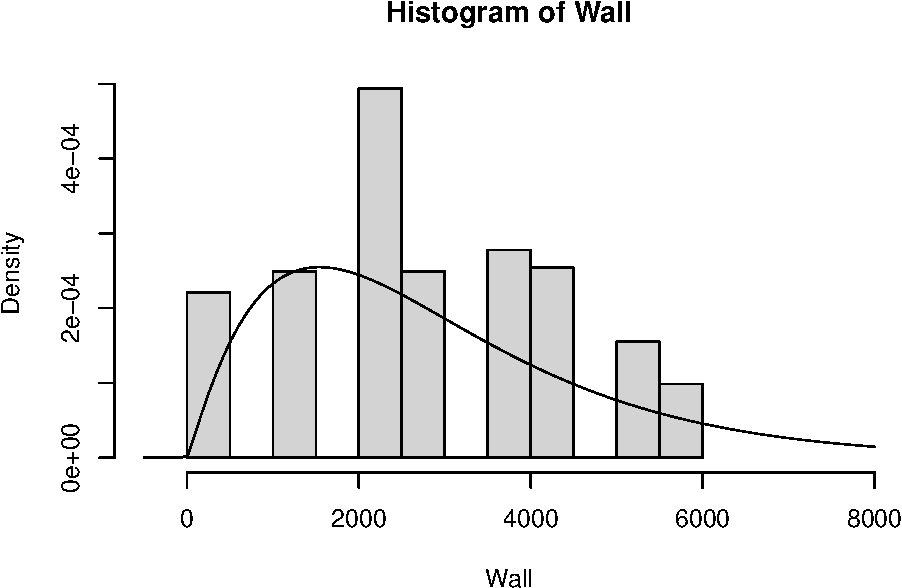
\includegraphics[width=0.8\linewidth]{resources/figs/flanders_wallonia-2} \end{center}

\begin{verbatim}
## [1] 0.05892352
\end{verbatim}

\begin{verbatim}
## [1] 0.0001358382
\end{verbatim}

    \hypertarget{question-1}{%
    \section{Question 1}\label{question-1}}

    Let \(\theta_k:= (\mu_k, \phi_k)\) be the set of parameters for a
    HNI with respect to region \(k\).

    \hypertarget{a-theoretical-probability}{%
    \subsection{(a) Theoretical
    probability}\label{a-theoretical-probability}}

    Let \(X\) be the monthly net income of 1123 Belgian households net
    income (HNI) older than 30 years. Regardless the 2 regions
    (\(k=\{1,2\}\) wrt Flanders and Wallonnia, respectively), is assumed
    it follows a Gamma distribution. It can be reparametrised in terms
    of its mean \(\mu\) and dispersion parameter \(\phi\) with the
    following trick:

    \[
    \begin{split}
    \text{shape: } \kappa & = \frac{1}{\phi} \\
    \text{rate: } \lambda & = \frac{1}{\phi\; \mu}
    \end{split}
    \]

    For both regions \(k=\{1,2\}\): This gives

    \[
    f(x_k) = \frac{(\phi_k\mu_k)^{-1/\phi_k}}{\Gamma(\phi_k^{-1})} \
    x_k^{1/\phi_k-1} \exp{(\frac{-x_k}{\phi_k \mu_k})}
    \]

    Then, the probability to fall into a certain HNI interval \(I\) is:

    \[
    P( x_k \in I_j) =\int_{I_j} \frac{(\phi_k \mu_k)^{-1/\phi_k}}{\Gamma(\phi_k^{-1})} x_k^{1/\phi_k-1} \exp{(\frac{-x_k}{\phi_k \mu_k})}\ \diff{x}
    \]

    Using CDF writing, for a region \(k\) ,

    \[
    p_j =
    \begin{cases}
     F(x_{j}, \kappa, \lambda) \ \text{if j =1}\\
     F(x_{j+1}, \kappa, \lambda) - F(x_{j}, \kappa, \lambda) \ \text{if} \ j \in \{2,..9\}\\
     1 - F(x_{j}, \kappa, \lambda) \ \text{if j =10}\\
    \end{cases}
    \]

    \[
    p_j =
    \begin{cases}
     \frac{1}{\Gamma(\kappa)} \gamma(\kappa, \lambda x_j)  \ \text{if j =1}\\
      \frac{1}{\Gamma(\kappa)} \Big(\gamma(\kappa, \lambda x_{j+1}) - \gamma(\kappa, \lambda x_j)  \Big)   \ \text{if} j \in \{2,..9\}\\
     1- \frac{1}{\Gamma(\kappa)} \gamma(\kappa, \lambda x_j)  \ \text{if j =10}\\
    \end{cases}
    \] In terms of \(\mu\) and \(\phi\) \[
    p_j =
    \begin{cases}
     \frac{1}{\Gamma(\phi^{-1})} \gamma(\phi^{-1}, (\mu \phi)^{-1} x_j)  \ \text{if j =1}\\
      \frac{1}{\Gamma(\phi^{-1})} \Big(\gamma(\phi^{-1}, (\mu \phi)^{-1}x_{j+1}) - \gamma(\kappa, (\mu \phi)^{-1} x_j)  \Big)   \ \text{if} j \in \{2,..9\}\\
     1- \frac{1}{\Gamma(\phi^{-1})} \gamma(\phi^{-1}, (\mu \phi)^{-1} x_j)  \ \text{if j =10}\\
    \end{cases}
    \]

    \[
    p_j =
    \begin{cases}
     \frac{1}{\Gamma(\phi^{-1})} \int^{(\mu \phi)^{-1} x_j}_0 t^{\phi^{-1}-1} e^{-t} \diff{t}   \ \text{if j =1}\\
      \frac{1}{\Gamma(\phi^{-1})} \int^{(\mu \phi)^{-1}x_{j+1}}_{ (\mu \phi)^{-1} x_j} t^{\phi^{-1}-1} e^{-t} \diff{t}  \ \text{if} j \in \{2,..9\}\\
     \frac{1}{\Gamma(\phi^{-1})} \int^{+ \infty}_{(\mu \phi)^{-1}x_j} t^{\phi^{-1}-1} e^{-t} \diff{t}  \ \text{if j =10}\\
    \end{cases}
    \]

    \hypertarget{b-theoretical-expression-for-the-likelihood}{%
    \subsection{(b) Theoretical expression for the
    likelihood}\label{b-theoretical-expression-for-the-likelihood}}

    On behalf of writing simplicity, the region index is removed. Since
    the frequency distribution in a given region is multinomial, i.e.~

    We have, writing \(P:=(p{1},..,p_{10})\) and
    \(X:= (X_{1},... X_{10})\):

    \[
    \begin{split}
    X | P  \sim \text{Mul}(N,P)  & = \frac{x!}{x_{1}! \, ... \, x_{10}! } p_1^{x_1} \times ... \times p_{10}^{x_{10}} \; \text{when} \sum_{j=1}^{10} p_j = 1 \\
    &=0 \; \text{otherwise}
    \end{split}
    \]

    Up to a multiplicative constant, the likelihood can be written as
    follow:

    \[
    \begin{split}
    L(\theta_k, D_k) = P (D_k | \mu_k, \phi_k) \propto \prod_{j=1}^{10} p_{k,j}^{x_{k,j}}
    \end{split}
    \]

    \hypertarget{taking-approximation}{%
    \subsection{Taking approximation}\label{taking-approximation}}

    \(p_j\) corresponds to the area in the \(j^{\text{th}}\) interval.
    One can take the approximation mean the
    mean,e.g.~\(x_{Flanders,3} = (1500+1800)/2 = 1650\) ? On can
    approximate that with \(f(x_i) \Delta\) where \(\Delta\) is the unit
    of measurement.

    \[
    \begin{split}
    p_j =P(x_j - \frac{\Delta_j}{2} < x_j <x_j + \frac{\Delta_j}{2} ) & \approx f(x_j) \Delta_j \\
    & \approx \frac{1}{\Gamma(\phi_k^{-1})} \big( \phi_k \mu \big)^{-1/\phi_k} x_j^{\frac{1}{\phi_k}-1} \exp{(\frac{-x_j}{\phi_k \mu})} \Delta_j
    \end{split}
    \] This gives for the likelihood:

    \[
    \begin{split}
    P (D | \mu, \phi) & \propto \prod_{j=1}^{10}  x_j^{\frac{1}{\phi_k}-1} \exp{(\frac{-x_j}{\phi_k \mu})} \Delta_j \\
    & \propto \exp{(\frac{- \sum x_j}{\phi_k \mu})}  \prod_{j=1}^{10}  x_j^{\frac{1}{\phi_k}-1}  \Delta_j \\
    \end{split}
    \]

    \hypertarget{not-taking-approximation-but-the-cdf-differences}{%
    \subsection{Not taking approximation but the CDF
    differences}\label{not-taking-approximation-but-the-cdf-differences}}

    \[
    \begin{split}
    P(D| \kappa, \lambda) & \propto \big(\frac{1}{\Gamma(\kappa)}\big)^{\sum_{i=1} x_j} \gamma(x_1 , \kappa, \lambda)^{x_1} \Bigg[ \prod_{j=2}^9  \Big( \gamma(x_{j} , \kappa, \lambda)- \gamma(x_{j-1} , \kappa, \lambda)\Big)^{x_j}\Bigg] \big(1-\gamma(x_{10} , \kappa, \lambda)\big)^{x_{10}}  \\
    & \propto \big(\frac{1}{\Gamma(\kappa)}\big)^{\sum_{i=1} x_j}  \Bigg( \int_0^{\lambda x_1}  x^{\kappa-1} e^{-x} \diff x \Bigg)^{x_1}  \Bigg[ \prod_{j=2}^9 \Big( \int_{\lambda  x_j-1}^{\lambda x_{j}}  x^{\kappa-1} e^{-x} \diff x \Big)^{x_{j}}\Bigg] \Bigg( \int_{\lambda x_{10}}^{+\infty}  x^{\kappa-1} e^{-x} \diff x \Bigg)^{x_{10}}
    \end{split} 
    \]

    If we write
    \([0; x_1], [x_1; x_2], ..., [x_9; x_{10}], [x_{10}, +\infty]\) as
    \(I_1, I_2, ..., I_9\) and \(I_{10}\). The notation can be
    lightened. With respect to the region \(k\), this gives: \[
    P(D_k | \kappa_k, \lambda_k) \propto \big(\frac{1}{\Gamma(\kappa)}\big)^{\sum_{i=1} x_j}  \prod_{j=1}^{10} \Bigg( \int\limits_{\lambda_k I_j} x^{\kappa_k-1} e^{-x} \diff x \Bigg)^{x_{k,j}}
    \]

    Writing in terms of \(\mu_k\) and \(\phi_k\):

    \[
    P(D_k | \mu_k, \phi_k) \propto  \prod_{j=1}^{10} \Bigg( \frac{1}{\Gamma(\phi^{-1})} \int\limits_{ \frac{I_j}{\phi_k \mu_k}} x^{(\phi_k^{-1}-1)} e^{-x} \diff x \Bigg)^{x_{k,j}}
    \]

    \hypertarget{not-taking-approximation-but-with-pdf-definitions}{%
    \subsection{NOT taking approximation but with PDF
    definitions:}\label{not-taking-approximation-but-with-pdf-definitions}}

    \hypertarget{question-2-priors}{%
    \section{Question 2 : Priors}\label{question-2-priors}}

    \begin{itemize}
    \tightlist
    \item
      Statement 1: we are at 95\% convinced that the mean net monthly
      household income in a given region is in the interval (2400,
      3600). If one assumes a normal distribution for the mean \(\mu_k\)
      (à justifier), then it is possible to get a prior of the
      distriubtion for both regions:
    \end{itemize}

    For both regions \(\mu_0 = 3000\). Then, to get the standard
    deviation:

    \[
    \begin{split}
    & 3000 - t_{(n_k-1, 1-\alpha/2)} \frac{s_k}{\sqrt{n_k}} = 2400 \\
    \rightarrow  & \hat{\sigma}_0 = \frac{s_k}{\sqrt{n_k}}= \frac{600}{t_{(n_k-1, 1-\alpha/2)}}
    \end{split}
    \]

    \(\hat{\sigma}_{Fl} = 306\)

    So we have \[\mu \sim N(\mu_0= 3000, \sigma_0 =306)\]

    \[
    \begin{split}
     \pi(\mu) \propto \sigma_0^{-1/2} \exp{ \big(-\frac{1}{2\sigma_0^2}(\mu-\mu_0)^2\big) }
    \end{split}
    \]

    \begin{itemize}
    \tightlist
    \item
      dispersion parameter:
    \end{itemize}

    If one considers that the parameter can be in any point within the
    interval (0.0, 10.0) with the same probability, then one could say
    that it follows a uniform distribution between those to interval

    \[
    \phi_k \sim U (a=0,b=10) \propto 1_{0,10}
    \]

    Using the entropy theorem, the conjugate prior would be the product
    of the two last quantity:

    \[
    \begin{split} 
    \text{prior:}  P(\mu_k, \phi_k) & = P(\mu_k) \ P(\phi_k) \\
    & \propto \sigma_0^{-1/2} \exp{ \big(-\frac{1}{2\sigma_0^2}(\mu-\mu_0)^2\big) } 1_{0;10}
    \end{split}
    \]

    \hypertarget{question-3}{%
    \section{Question 3}\label{question-3}}

    \hypertarget{question-3a-posterior}{%
    \subsection{Question 3a: posterior}\label{question-3a-posterior}}

    \hypertarget{with-approximation}{%
    \subsubsection{With approximation}\label{with-approximation}}

    \(\sigma^2 = \phi \mu^2\)

    \[
    \begin{split}
    P(\mu, \phi | D) & \propto \exp{(\frac{- \sum x_j}{\phi_k \mu})}  \prod_{j=1}^{10}  x_j^{\frac{1}{\phi_k}-1}  \Delta_j \sigma^{-1/2} \exp{ \big(-\frac{1}{2\sigma^2}(\bar{x}_k-\mu)^2\big) } 1_{0,10} \\ 
    & \propto \exp{(\frac{- \sum x_j}{\phi_k \mu})}  \prod_{j=1}^{10}  x_j^{\frac{1}{\phi_k}-1}  \Delta_j (\frac{1}{\sqrt{\phi} \mu}) \exp{ \big(-\frac{1}{2 \phi \mu^2}(\bar{x}_k-\mu)^2\big) } 1_{0,10} \\
    \end{split}
    \]

    \hypertarget{without-approximation}{%
    \subsubsection{Without approximation}\label{without-approximation}}

    \[
    \begin{split}
    P(\mu_k, \phi_k | D) \propto  \Bigg( \prod_{j=1}^{10} \Bigg( \frac{1}{\Gamma(\phi^{-1})} \int\limits_{ \frac{I_j}{\phi_k \mu_k}} x^{(\phi_k^{-1}-1)} e^{-x} \diff x \Bigg)^{x_{k,j}} \Bigg)  \sigma_0^{-1/2} \exp{ \big(-\frac{1}{2\sigma_0^2}(\mu-\mu_0)^2\big) } 1_{0;10}
    \end{split}
    \]

    \hypertarget{b}{%
    \subsection{3.b}\label{b}}

    the log likelihood is, up to an additive constant: \[
    \begin{split}
    l(\mu,\phi) & \propto  \sum_{j=1}^{10} x_j \ln{\Bigg(\frac{1}{\Gamma(\phi^{-1})} \int\limits_{ \frac{I_j}{\phi_k \mu_k}} x^{(\phi_k^{-1}-1)} e^{-x} \diff x \Bigg)}
    \end{split}
    \] so the log-posterior is:

    \[
    h(\mu,\phi) \propto  l(\mu,\phi) + \ln(\pi(\mu,\phi))
    \]

    \[
    h(\mu,\phi) = C^t +  \sum_j x_j \ln{\big(F(\mu,\phi,x_{j+1})-F(\mu,\phi,x_{j})  \big)} - \frac{1}{2 \sigma_0^2} (\mu-\mu_0)^2
    \]

\begin{verbatim}
##     shape 
## -1755.997
\end{verbatim}

\begin{verbatim}
##     shape 
## -956.3546
\end{verbatim}

    \hypertarget{section}{%
    \section{4.}\label{section}}

    \hypertarget{estimation}{%
    \subsection{Estimation}\label{estimation}}

    Start from the log-posterior \(h(\mu_k, \phi_k)\). One assumes the
    distribution is unimodale then, if it is normally distributed, then
    the mode=mean, which means that the mean can be found by optimizing
    the log-likelihood with respect to its parameters. (aussi assumer
    \(\mu\) et \(\phi\) indépendant?? ), then blablabla (expliquez avec
    hessienne).

    Based on
    \url{http://www.sumsar.net/blog/2013/11/easy-laplace-approximation/\#}:\textasciitilde:text=Laplace\%20Approximation\%20of\%20Posterior\%20Distributions\&text=Laplace\%20approximation\%20is\%20a\%20method,the\%20posterior\%20at\%20the\%20mode.

    \hypertarget{flanders}{%
    \subsubsection{Flanders}\label{flanders}}

\begin{verbatim}
##      mu     phi 
## 3698.91    0.22
\end{verbatim}

\begin{verbatim}
##           mu  phi
## mu  3952.206 0.04
## phi    0.040 0.00
\end{verbatim}

    \begin{center}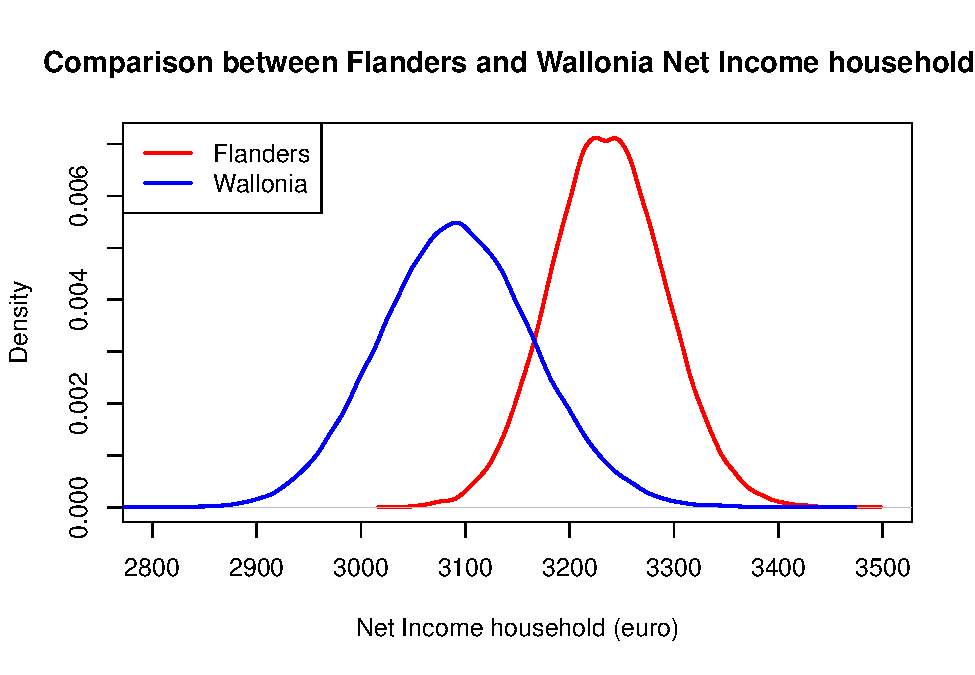
\includegraphics[width=0.8\linewidth]{resources/figs/unnamed-chunk-7-1} \end{center}

    \begin{center}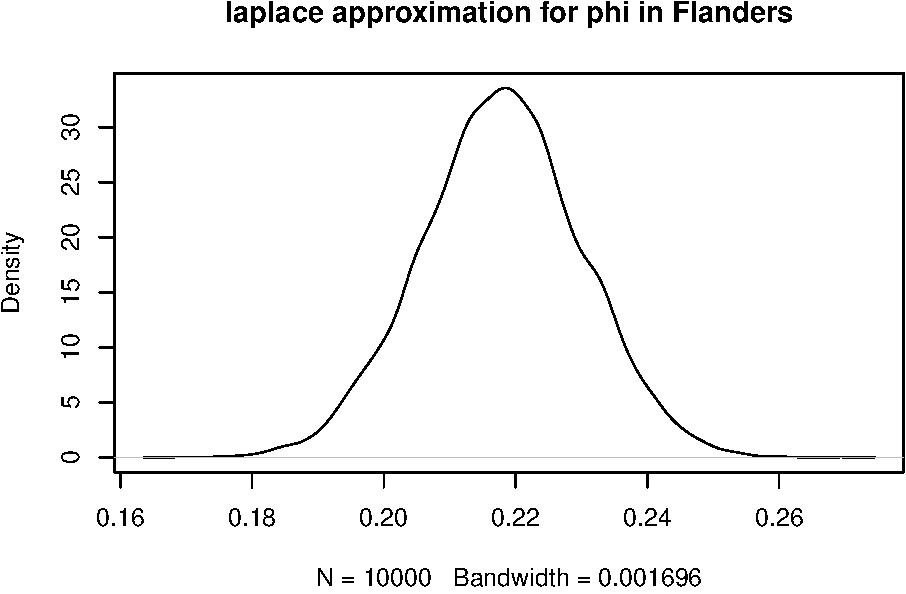
\includegraphics[width=0.8\linewidth]{resources/figs/unnamed-chunk-7-2} \end{center}

    \hypertarget{wallonia}{%
    \subsubsection{Wallonia}\label{wallonia}}

\begin{verbatim}
##      mu     phi 
## 3525.57    0.23
\end{verbatim}

\begin{verbatim}
##           mu   phi
## mu  6639.722 0.038
## phi    0.038 0.000
\end{verbatim}

    \begin{center}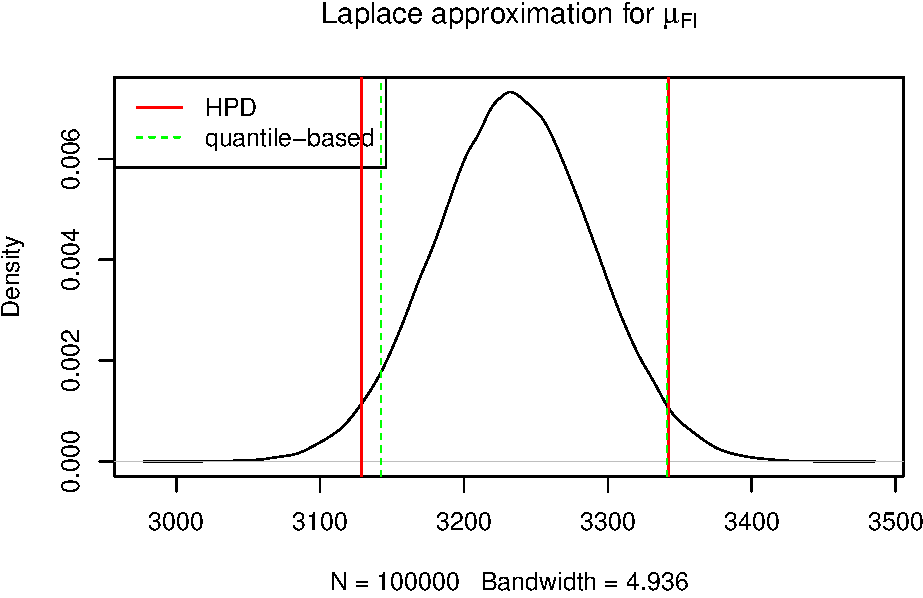
\includegraphics[width=0.8\linewidth]{resources/figs/unnamed-chunk-9-1} \end{center}

    \begin{center}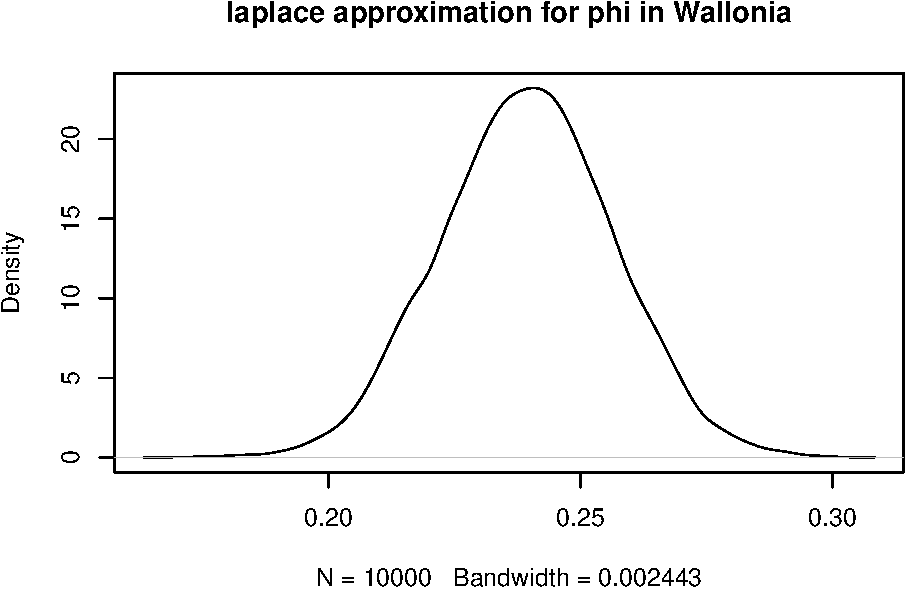
\includegraphics[width=0.8\linewidth]{resources/figs/unnamed-chunk-9-2} \end{center}

    \hypertarget{credible-intervals-laplce-approximation}{%
    \subsection{Credible intervals Laplce
    approximation}\label{credible-intervals-laplce-approximation}}

    \hypertarget{flanders-1}{%
    \subsubsection{Flanders}\label{flanders-1}}

    The credible region is given here below:

    \begin{center}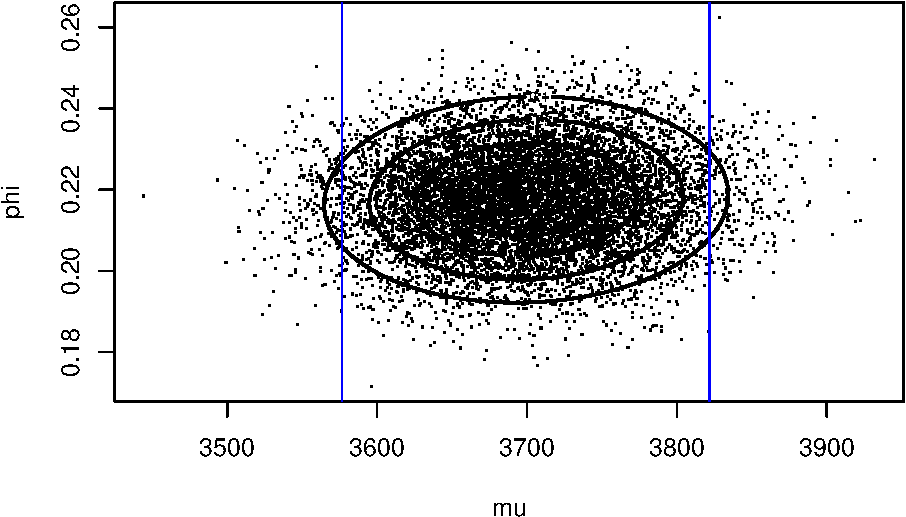
\includegraphics[width=0.8\linewidth]{resources/figs/unnamed-chunk-11-1} \end{center}

    We needs to get the credible interval for \(\mu\). This means that
    we needs the marginal posterior distribution:

    \[
    P(\mu| D) \propto \int p(\mu, \phi |D) \diff \phi
    \]

    It can be shown that the marginal (univariate) distribution of the
    bivariate Gaussian distribution \(N\big( \mu_\theta, \Sigma)\) with
    \(\mu_\theta = (E(\mu), E(\phi) )\) and

    \[
    \Sigma =
    \begin{pmatrix}
    \sigma_\mu & \sigma_{\mu,\phi} \\
    \sigma_{\phi,\mu} & \sigma_\phi
    \end{pmatrix}
    \] also follows a normal distribution. See
    \href{https://paolomaccallini.com/2018/06/20/bivariate-normal-distribution/}{here}.
    Hence, for \(\mu\), one has:

    \[\mu|D \sim N(E(\mu),\sigma_\mu) \] We needs that \(95\%\) of the
    marginal posterior to fall into the interval for Flanders:

    \begin{center}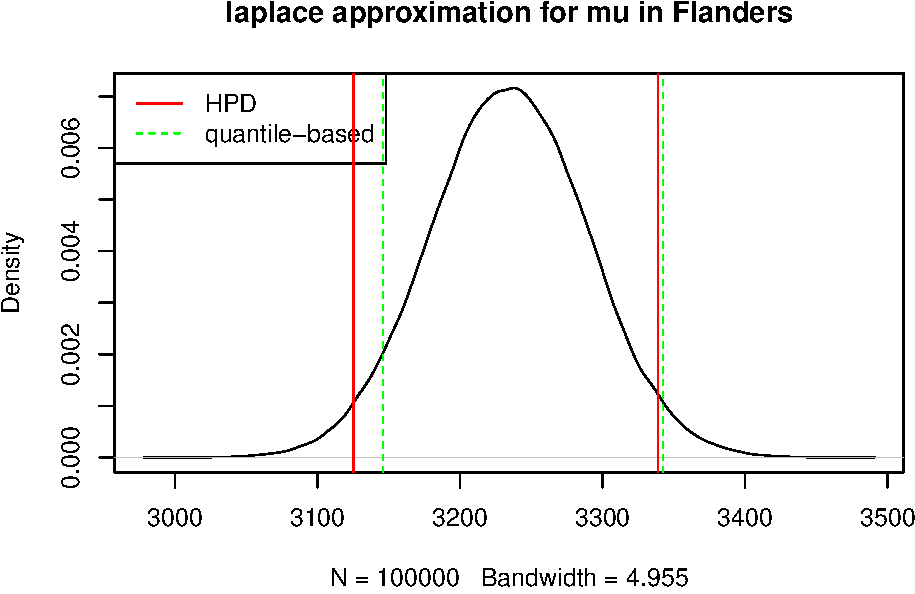
\includegraphics[width=0.8\linewidth]{resources/figs/unnamed-chunk-12-1} \end{center}

    Il faut encore faire pour phi de la Flandre

    \hypertarget{question-5}{%
    \section{Question 5}\label{question-5}}

    \hypertarget{a}{%
    \subsection{(a)}\label{a}}

\begin{verbatim}
##             [,1] [,2] [,3] [,4] [,5]
## [1,] 3089.943960   NA   NA   NA   NA
## [2,]    0.399687   NA   NA   NA   NA
\end{verbatim}

\begin{verbatim}
## Acceptance rate :  21%
\end{verbatim}

\begin{verbatim}
##        mu            phi        
##  Min.   :3464   Min.   :0.1771  
##  1st Qu.:3661   1st Qu.:0.2111  
##  Median :3701   Median :0.2187  
##  Mean   :3701   Mean   :0.2192  
##  3rd Qu.:3743   3rd Qu.:0.2270  
##  Max.   :3953   Max.   :0.2832
\end{verbatim}

    Il va falloir comparer ça avec la Laplace approximation

    \hypertarget{b-diagnostic}{%
    \subsection{(b) diagnostic}\label{b-diagnostic}}

    difficult to say if mixing is good while checking the trace (?)

    \begin{center}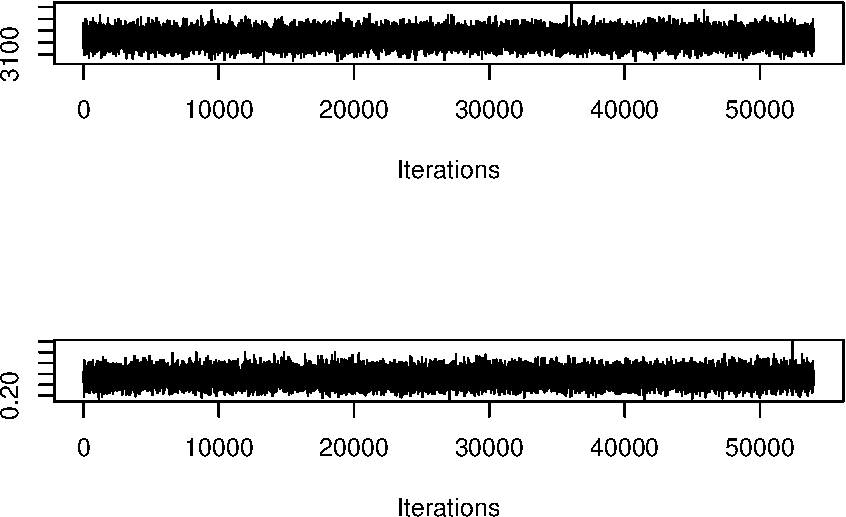
\includegraphics[width=0.8\linewidth]{resources/figs/unnamed-chunk-14-1} \end{center}

    \begin{center}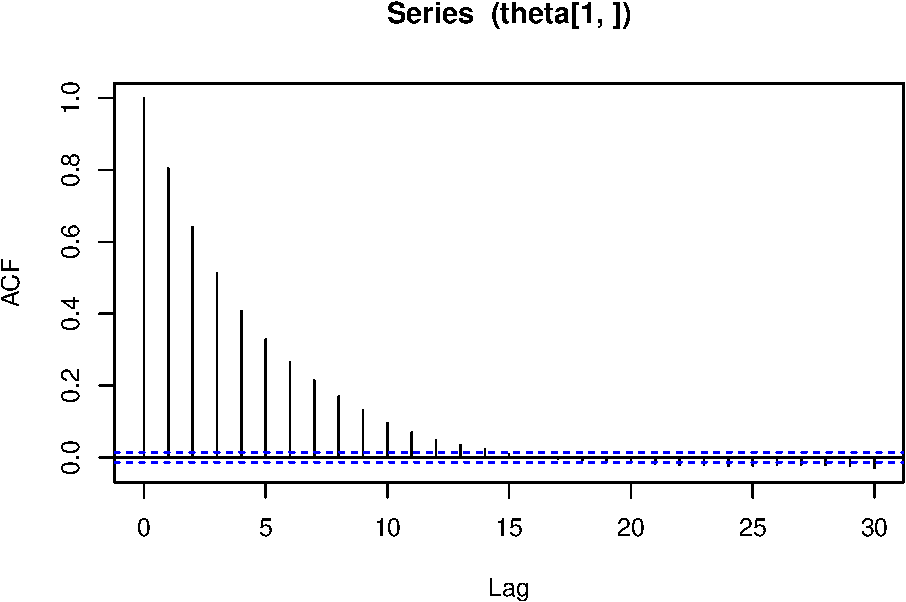
\includegraphics[width=0.8\linewidth]{resources/figs/unnamed-chunk-15-1} \end{center}

    \begin{center}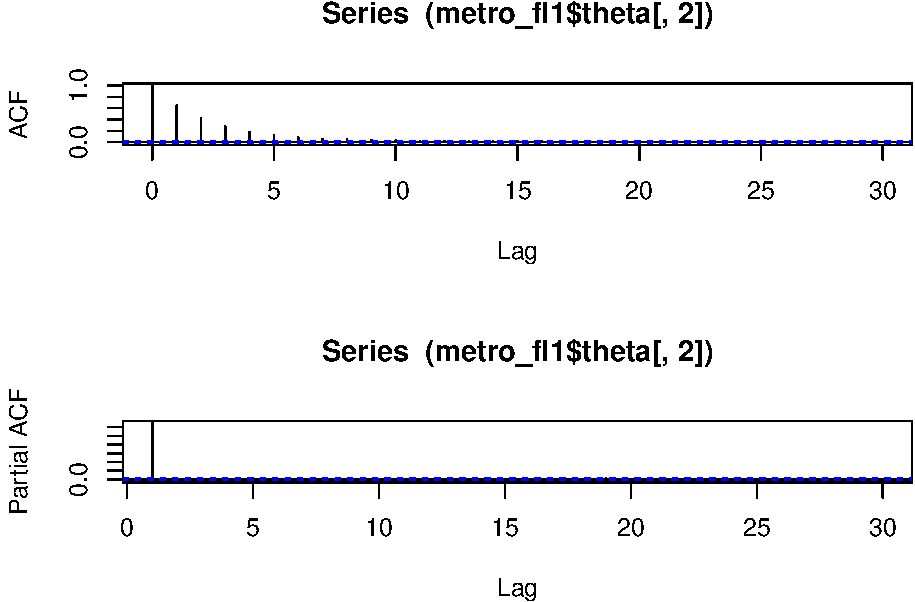
\includegraphics[width=0.8\linewidth]{resources/figs/unnamed-chunk-15-2} \end{center}

\begin{verbatim}
##       mu      phi 
## 2540.062 2313.226
\end{verbatim}

    Assesment from a single chain

\begin{verbatim}
## 
## Fraction in 1st window = 0.1
## Fraction in 2nd window = 0.5 
## 
##      mu     phi 
## 0.06931 0.41394
\end{verbatim}

    \begin{center}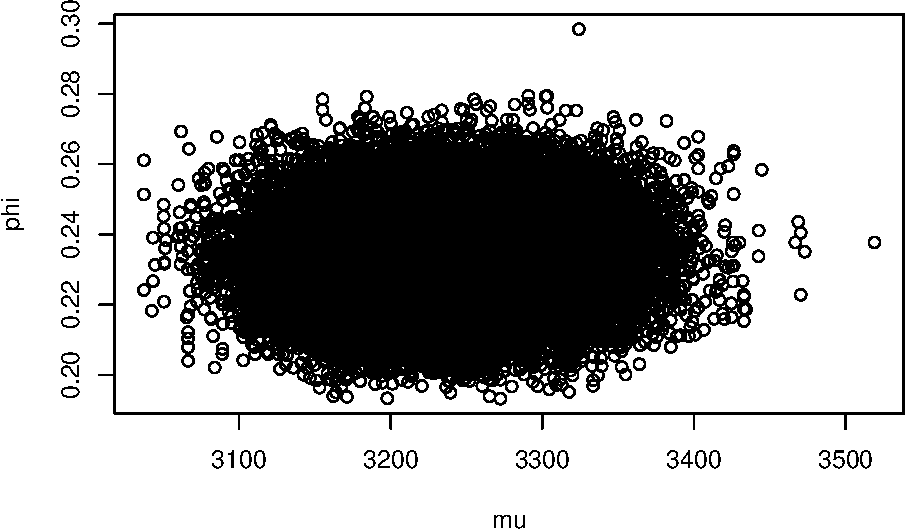
\includegraphics[width=0.8\linewidth]{resources/figs/unnamed-chunk-16-1} \end{center}

    Except for one, they ye all into the confidence interval. Hence,
    there is no reason to think that the chain needs to be truncated or
    the chain to be made longer.

    \hypertarget{c-credible-intervals-for-mu1}{%
    \subsection{(c) Credible intervals for
    mu1}\label{c-credible-intervals-for-mu1}}

    Bon là, y a tout en dessous

    Metropolis:

    \begin{center}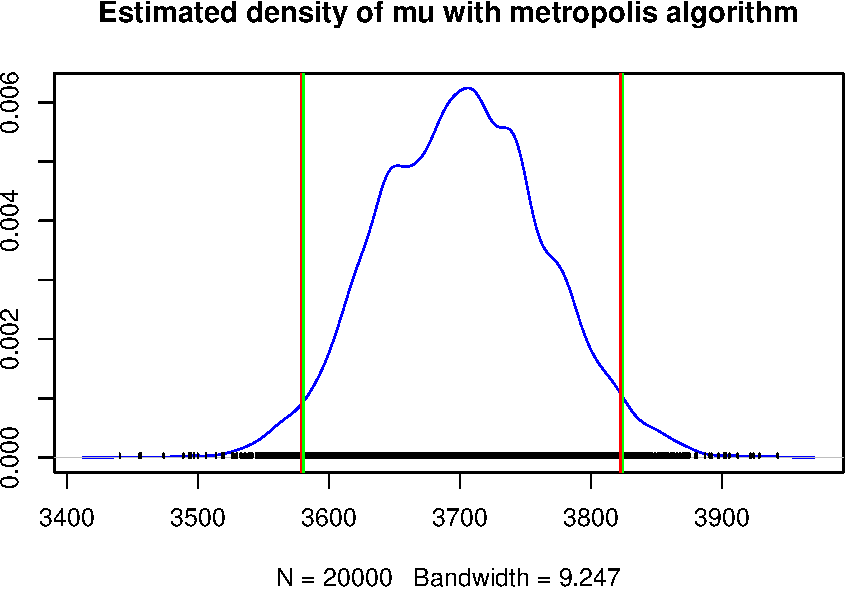
\includegraphics[width=0.8\linewidth]{resources/figs/unnamed-chunk-17-1} \end{center}

    \begin{center}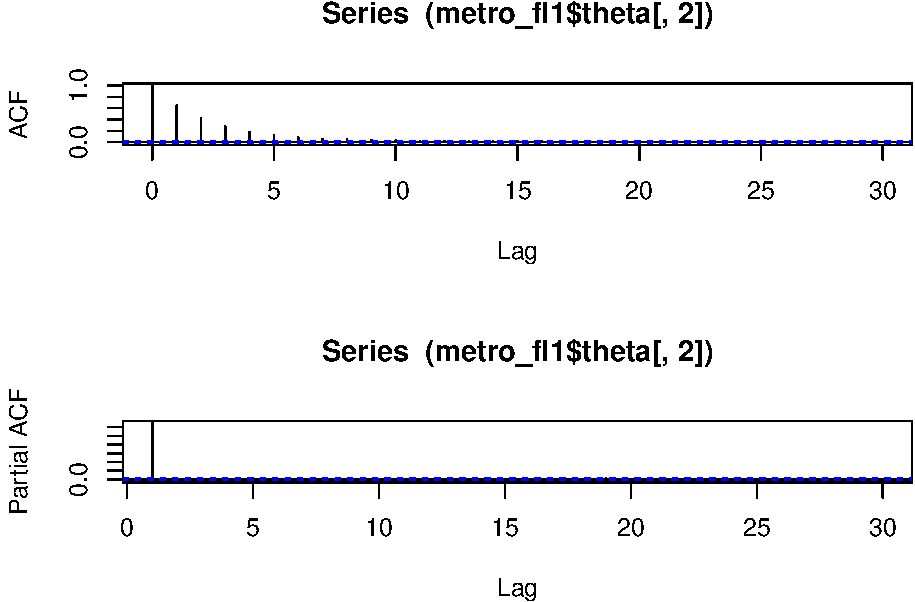
\includegraphics[width=0.8\linewidth]{resources/figs/unnamed-chunk-17-2} \end{center}

    Comparison: voir les deux graphes et chopper les valeurs

    \appendix

    \hypertarget{appendix}{%
    \section{Appendix}\label{appendix}}

    \hypertarget{figures}{%
    \subsection{Figures}\label{figures}}

    \hypertarget{code}{%
    \subsection{Code}\label{code}}

    \bigskip
    \begin{mdframed}[style=thicc, frametitle=Note, frametitlebackgroundcolor=black!30]
      For reproducibility purposes, the complete R project containing the source code and the results is available on \href{https://github.com/AdrienKinart/LSTAT2130BayesianProject}{github.com}.
    \end{mdframed}


\end{document}
